\documentclass{standalone}
\usepackage{tikz}
\usetikzlibrary{patterns, positioning}
\usepackage[sfdefault]{ClearSans} %% option 'sfdefault' activates Clear Sans as the default text font
\usepackage[T1]{fontenc}

\begin{document}
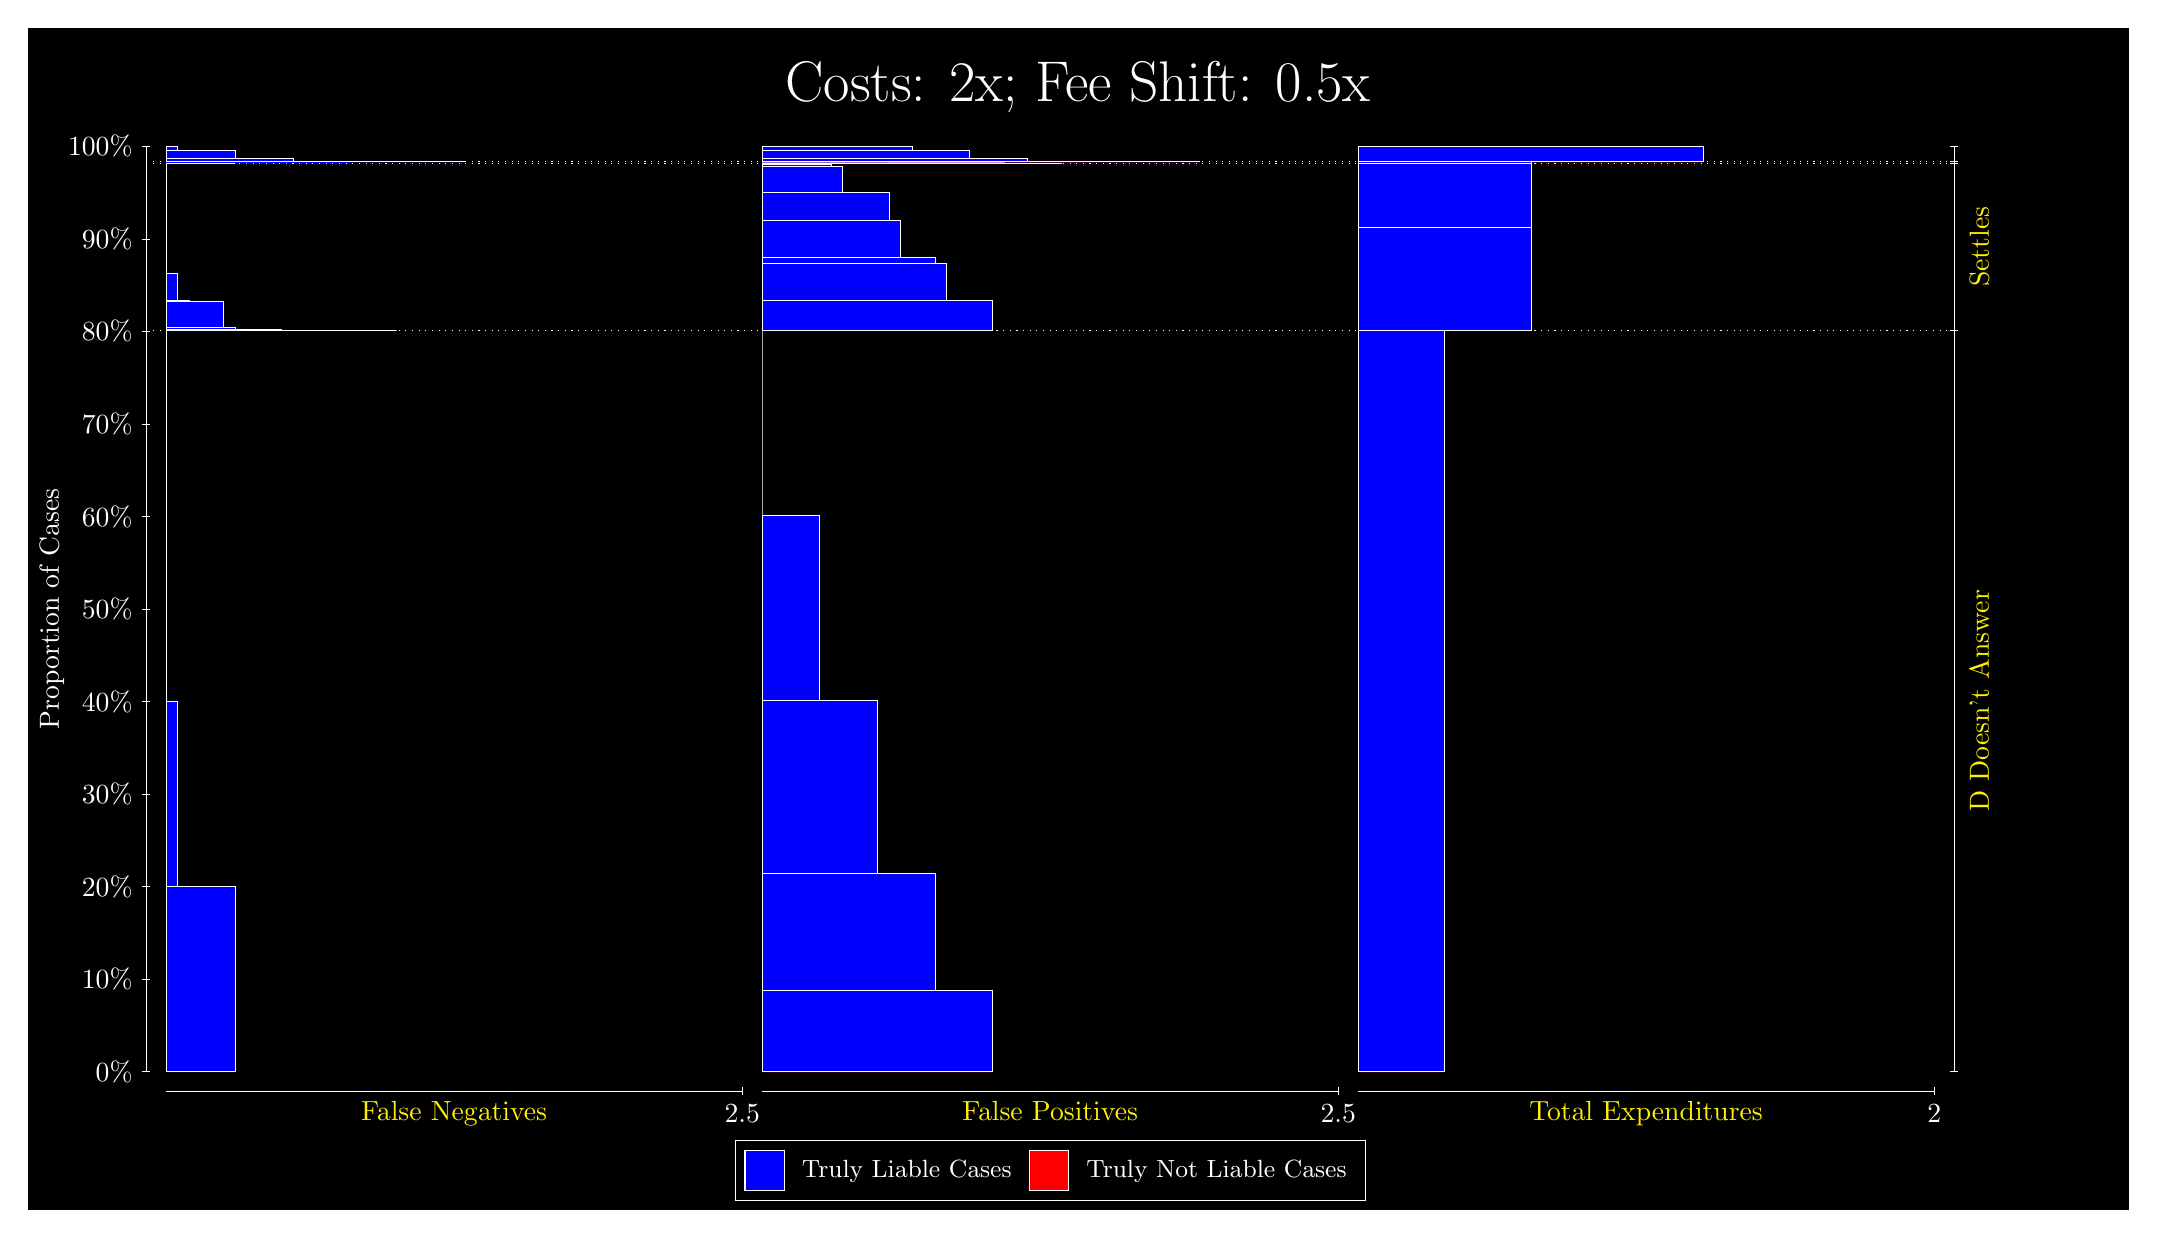
\begin{tikzpicture}
\draw[fill=black] (0,0) rectangle (26.667,15);
\draw[text=white] (0,13.5) rectangle (26.667,15) node[midway] {\huge Costs: 2x; Fee Shift: 0.5x};
\draw[white, very thin] (1.5,1.75) -- (1.5,13.5);
\node[rotate=90, text=white, anchor=center] at (0.3, 7.625) {Proportion of Cases};
\draw[white, very thin] (1.45,1.75) -- (1.55,1.75);
\node[text=white, anchor=east] at (1.45, 1.75) {0\%};
\draw[white, very thin] (1.45,2.925) -- (1.55,2.925);
\node[text=white, anchor=east] at (1.45, 2.925) {10\%};
\draw[white, very thin] (1.45,4.1) -- (1.55,4.1);
\node[text=white, anchor=east] at (1.45, 4.1) {20\%};
\draw[white, very thin] (1.45,5.275) -- (1.55,5.275);
\node[text=white, anchor=east] at (1.45, 5.275) {30\%};
\draw[white, very thin] (1.45,6.45) -- (1.55,6.45);
\node[text=white, anchor=east] at (1.45, 6.45) {40\%};
\draw[white, very thin] (1.45,7.625) -- (1.55,7.625);
\node[text=white, anchor=east] at (1.45, 7.625) {50\%};
\draw[white, very thin] (1.45,8.8) -- (1.55,8.8);
\node[text=white, anchor=east] at (1.45, 8.8) {60\%};
\draw[white, very thin] (1.45,9.975) -- (1.55,9.975);
\node[text=white, anchor=east] at (1.45, 9.975) {70\%};
\draw[white, very thin] (1.45,11.15) -- (1.55,11.15);
\node[text=white, anchor=east] at (1.45, 11.15) {80\%};
\draw[white, very thin] (1.45,12.325) -- (1.55,12.325);
\node[text=white, anchor=east] at (1.45, 12.325) {90\%};
\draw[white, very thin] (1.45,13.5) -- (1.55,13.5);
\node[text=white, anchor=east] at (1.45, 13.5) {100\%};

\draw[white, very thin] (24.457,1.75) -- (24.457,13.5);
\draw[white, very thin] (24.407,1.75) -- (24.507,1.75);
\node[anchor=west] at (24.407, 1.75) {};
\draw[white, very thin] (24.407,11.164) -- (24.507,11.164);
\node[anchor=west] at (24.407, 11.164) {};
\draw[white, very thin] (24.407,13.285) -- (24.507,13.285);
\node[anchor=west] at (24.407, 13.285) {};
\draw[white, very thin] (24.407,13.304) -- (24.507,13.304);
\node[anchor=west] at (24.407, 13.304) {};
\draw[white, very thin] (24.407,13.5) -- (24.507,13.5);
\node[anchor=west] at (24.407, 13.5) {};

\draw[white, very thin, fill=blue] (1.75,1.75) rectangle (2.6283,4.0999);
\draw[white, very thin, fill=blue] (1.75,4.0999) rectangle (1.8964,6.4487);
\draw[white, very thin, fill=red] (1.75,6.4487) rectangle (1.75,6.4487);
\draw[white, very thin, fill=blue] (1.75,6.4487) rectangle (1.75,11.164);
\draw[white, very thin, fill=blue] (1.75,11.164) rectangle (4.6775,11.164);
\draw[white, very thin, fill=blue] (1.75,11.164) rectangle (4.092,11.164);
\draw[white, very thin, fill=blue] (1.75,11.164) rectangle (3.9457,11.164);
\draw[white, very thin, fill=blue] (1.75,11.164) rectangle (3.5065,11.164);
\draw[white, very thin, fill=blue] (1.75,11.164) rectangle (3.3602,11.164);
\draw[white, very thin, fill=blue] (1.75,11.164) rectangle (3.2138,11.176);
\draw[white, very thin, fill=blue] (1.75,11.176) rectangle (2.7746,11.176);
\draw[white, very thin, fill=blue] (1.75,11.176) rectangle (2.6283,11.205);
\draw[white, very thin, fill=blue] (1.75,11.205) rectangle (2.4819,11.538);
\draw[white, very thin, fill=blue] (1.75,11.538) rectangle (2.0428,11.539);
\draw[white, very thin, fill=blue] (1.75,11.539) rectangle (1.8964,11.892);
\draw[white, very thin, fill=red] (1.75,11.892) rectangle (1.75,11.892);
\draw[white, very thin, fill=blue] (1.75,11.892) rectangle (1.75,13.285);
\draw[white, very thin, fill=blue] (1.75,13.285) rectangle (2.6283,13.285);
\draw[white, very thin, fill=blue] (1.75,13.285) rectangle (1.8964,13.285);
\draw[white, very thin, fill=red] (1.75,13.285) rectangle (1.75,13.285);
\draw[white, very thin, fill=blue] (1.75,13.285) rectangle (1.75,13.304);
\draw[white, very thin, fill=blue] (1.75,13.304) rectangle (5.5558,13.304);
\draw[white, very thin, fill=blue] (1.75,13.304) rectangle (4.8239,13.304);
\draw[white, very thin, fill=blue] (1.75,13.304) rectangle (4.092,13.306);
\draw[white, very thin, fill=blue] (1.75,13.306) rectangle (3.3602,13.352);
\draw[white, very thin, fill=blue] (1.75,13.352) rectangle (2.6283,13.352);
\draw[white, very thin, fill=blue] (1.75,13.352) rectangle (2.6283,13.45);
\draw[white, very thin, fill=blue] (1.75,13.45) rectangle (1.8964,13.45);
\draw[white, very thin, fill=blue] (1.75,13.45) rectangle (1.8964,13.496);
\draw[white, very thin, fill=red] (1.75,13.496) rectangle (1.75,13.496);
\draw[white, very thin, fill=blue] (1.75,13.496) rectangle (1.75,13.5);
\draw[white, very thin, fill=red] (9.3189,1.75) rectangle (12.246,1.75);
\draw[white, very thin, fill=blue] (9.3189,1.75) rectangle (12.246,2.7801);
\draw[white, very thin, fill=blue] (9.3189,2.7801) rectangle (11.515,4.2655);
\draw[white, very thin, fill=blue] (9.3189,4.2655) rectangle (10.783,6.4657);
\draw[white, very thin, fill=blue] (9.3189,6.4657) rectangle (10.051,8.8145);
\draw[white, very thin, fill=blue] (9.3189,8.8145) rectangle (9.3189,11.164);
\draw[white, very thin, fill=red] (9.3189,11.164) rectangle (12.246,11.164);
\draw[white, very thin, fill=blue] (9.3189,11.164) rectangle (12.246,11.546);
\draw[white, very thin, fill=red] (9.3189,11.546) rectangle (11.661,11.546);
\draw[white, very thin, fill=blue] (9.3189,11.546) rectangle (11.661,12.015);
\draw[white, very thin, fill=blue] (9.3189,12.015) rectangle (11.515,12.089);
\draw[white, very thin, fill=red] (9.3189,12.089) rectangle (11.075,12.089);
\draw[white, very thin, fill=blue] (9.3189,12.089) rectangle (11.075,12.557);
\draw[white, very thin, fill=blue] (9.3189,12.557) rectangle (10.929,12.911);
\draw[white, very thin, fill=blue] (9.3189,12.911) rectangle (10.783,12.911);
\draw[white, very thin, fill=blue] (9.3189,12.911) rectangle (10.344,13.244);
\draw[white, very thin, fill=blue] (9.3189,13.244) rectangle (10.197,13.273);
\draw[white, very thin, fill=blue] (9.3189,13.273) rectangle (10.051,13.273);
\draw[white, very thin, fill=blue] (9.3189,13.273) rectangle (9.6116,13.285);
\draw[white, very thin, fill=blue] (9.3189,13.285) rectangle (9.4652,13.285);
\draw[white, very thin, fill=blue] (9.3189,13.285) rectangle (9.3189,13.285);
\draw[white, very thin, fill=red] (9.3189,13.285) rectangle (13.125,13.285);
\draw[white, very thin, fill=blue] (9.3189,13.285) rectangle (13.125,13.285);
\draw[white, very thin, fill=blue] (9.3189,13.285) rectangle (12.393,13.293);
\draw[white, very thin, fill=blue] (9.3189,13.293) rectangle (11.661,13.304);
\draw[white, very thin, fill=blue] (9.3189,13.304) rectangle (10.929,13.304);
\draw[white, very thin, fill=blue] (9.3189,13.304) rectangle (10.197,13.304);
\draw[white, very thin, fill=red] (9.3189,13.304) rectangle (14.881,13.304);
\draw[white, very thin, fill=blue] (9.3189,13.304) rectangle (14.881,13.304);
\draw[white, very thin, fill=red] (9.3189,13.304) rectangle (14.149,13.304);
\draw[white, very thin, fill=blue] (9.3189,13.304) rectangle (14.149,13.304);
\draw[white, very thin, fill=red] (9.3189,13.304) rectangle (13.417,13.304);
\draw[white, very thin, fill=blue] (9.3189,13.304) rectangle (13.417,13.308);
\draw[white, very thin, fill=red] (9.3189,13.308) rectangle (12.686,13.308);
\draw[white, very thin, fill=blue] (9.3189,13.308) rectangle (12.686,13.354);
\draw[white, very thin, fill=red] (9.3189,13.354) rectangle (11.954,13.354);
\draw[white, very thin, fill=blue] (9.3189,13.354) rectangle (11.954,13.453);
\draw[white, very thin, fill=blue] (9.3189,13.453) rectangle (11.222,13.498);
\draw[white, very thin, fill=blue] (9.3189,13.498) rectangle (10.49,13.5);
\draw[white, very thin, fill=blue] (9.3189,13.5) rectangle (9.758,13.5);
\draw[white, very thin, fill=blue] (9.3189,13.5) rectangle (9.3189,13.5);
\draw[white, very thin, fill=red] (16.888,1.75) rectangle (17.986,1.75);
\draw[white, very thin, fill=blue] (16.888,1.75) rectangle (17.986,11.164);
\draw[white, very thin, fill=red] (16.888,11.164) rectangle (19.083,11.164);
\draw[white, very thin, fill=blue] (16.888,11.164) rectangle (19.083,12.472);
\draw[white, very thin, fill=red] (16.888,12.472) rectangle (19.083,12.472);
\draw[white, very thin, fill=blue] (16.888,12.472) rectangle (19.083,13.285);
\draw[white, very thin, fill=red] (16.888,13.285) rectangle (19.083,13.285);
\draw[white, very thin, fill=blue] (16.888,13.285) rectangle (19.083,13.304);
\draw[white, very thin, fill=red] (16.888,13.304) rectangle (21.279,13.304);
\draw[white, very thin, fill=blue] (16.888,13.304) rectangle (21.279,13.5);
\draw[white, dotted] (1.5,11.164) -- (24.457,11.164);
\draw[white, dotted] (1.5,13.285) -- (24.457,13.285);
\draw[white, dotted] (1.5,13.304) -- (24.457,13.304);
\draw[white, very thin] (1.75,1.5) -- (9.0689,1.5);
\node[text=yellow, anchor=north] at (5.4094, 1.5) {False Negatives};
\draw[white, very thin] (9.0689,1.45) -- (9.0689,1.55);
\node[text=white, anchor=north] at (9.0689, 1.45) {2.5};

\draw[white, very thin] (9.3189,1.5) -- (16.638,1.5);
\node[text=yellow, anchor=north] at (12.978, 1.5) {False Positives};
\draw[white, very thin] (16.638,1.45) -- (16.638,1.55);
\node[text=white, anchor=north] at (16.638, 1.45) {2.5};

\draw[white, very thin] (16.888,1.5) -- (24.207,1.5);
\node[text=yellow, anchor=north] at (20.547, 1.5) {Total Expenditures};
\draw[white, very thin] (24.207,1.45) -- (24.207,1.55);
\node[text=white, anchor=north] at (24.207, 1.45) {2};

\node[text=yellow, centered, rotate=90] at (24.777, 6.4572) {D Doesn't Answer};
\node[text=yellow, centered, rotate=90] at (24.777, 12.225) {Settles};



\draw (12.978300999999998,1.5) node[draw=none] (baseCoordinate) {};
\begin{scope}[align=center]
        \matrix[scale=0.5, draw=white, below=0.5cm of baseCoordinate, nodes={draw}, column sep=0.1cm]{
            \node[rectangle, draw, minimum width=0.5cm, minimum height=0.5cm, fill=blue] {}; &
            \node[draw=none, font=\small, text=white] (B) {Truly Liable Cases}; &
            \node[rectangle, draw, minimum width=0.5cm, minimum height=0.5cm, fill=red] {}; &
            \node[draw=none, font=\small, text=white] (B) {Truly Not Liable Cases}; \\
            };
\end{scope}

\end{tikzpicture}
\end{document}